\subsection{Forecasting for route selection}

Validation of v8 yielded 80/80 valid cells; the go decision passed and the test
yielded 192/192 valid cells.

Table~\ref{tab:v8primary} presents the comparisons in the pre-locked order.

\begin{table}[htbp]
\centering\small
\begin{tabularx}{\linewidth}{@{}Yp{1.8cm}p{3.4cm}p{1.7cm}@{}}
\toprule
\textbf{Comparison}&\textbf{Difference}&\textbf{95\% CI}&\textbf{Gate}\\\midrule
H1: \code{gnn-route} $-$ \code{lq-route}&0.66&[0.38, 1.00]&Met\\
H2: \code{gnn-route} $-$ \code{mlp-route}&0.38&[0.12, 0.67]&Met\\
H3: \code{gnn-route} $-$ \code{olsr-etx-fast}&5.75&[5.07, 6.45]&Met\\
\bottomrule
\end{tabularx}
\caption{Routing test: PDR in percentage points. Each comparison uses 40 fresh gradual blocks.}\label{tab:v8primary}
\end{table}


The primary endpoint was met and the subsequent steps follow the sequential gate
shown in the table. Route integrity was correct in 144/144 inspected episodes
and all technical checks passed.

H3 compares a centralized controller against a distributed protocol in a setting
where telemetry and commands are not transmitted as channel-contending packets.
The difference of 5.75 percentage points is therefore an upper bound for this
centralized configuration rather than the gain expected once signalling is fully
simulated; the corresponding signalling cost is 5.55~kB/s against 1.78~kB/s.

Table~\ref{tab:v8meanspaper} records the PDR, disconnected time and travelled
distance of each arm.

\begin{table}[htbp]
\centering\small
\begin{tabularx}{\linewidth}{@{}Yp{3.4cm}p{2.2cm}p{2.5cm}@{}}
\toprule
\textbf{Arm}&\textbf{PDR (\%, mean $\pm$ SD)}&\textbf{Disconnected (s)}&\textbf{Distance (m)}\\\midrule
\code{gnn-route}&96.01 $\pm$ 2.58&31.65&0.00\\
\code{lq-route}&95.35 $\pm$ 2.92&31.77&0.00\\
\code{mlp-route}&95.64 $\pm$ 2.68&31.77&0.00\\
\code{olsr-etx-fast}&90.26 $\pm$ 4.38&35.90&0.00\\
\bottomrule
\end{tabularx}
\caption{Descriptive statistics for the v8 gradual test; PDR mean and SD are per episode and the remaining columns are means. Distance is summed over relays and does not represent energy.}\label{tab:v8meanspaper}
\end{table}


On the same \code{lq-route} test traces, the MSE of the GNN, the MLP and the
EWMA is 0.0007846, 0.0011143 and 0.0012738 respectively. The number of
route-change commands over the whole test is 95 for the GNN, 208 for the MLP and
359 for the EWMA. The GNN minus EWMA difference in disconnected time is $-0.13$
seconds, 95\% CI [$-0.97$, $0.68$], which shows no clear reduction in
disconnection. The static context has a PDR near 100\% and a GNN minus EWMA
difference of zero over eight blocks. The background-flow PDR difference of GNN
minus EWMA is 0.005 percentage points, 95\% CI [$-0.119$, $0.123$], and is
descriptive only.

Whole-decision latency for the GNN has a median of 4.92~ms and a 95th percentile
of 13.83~ms; the EWMA median is 3.00~ms. These are server CPU measurements and
exclude telemetry and command transmission.

\subsection{Forecasting for motion triggering}

Validation of v9 yielded 80/80 valid cells; the go decision passed and the test
yielded 192/192 valid cells.

Table~\ref{tab:v9primary} presents the comparisons in the pre-locked order.

\begin{table}[htbp]
\centering\small
\begin{tabularx}{\linewidth}{@{}Yp{1.8cm}p{3.4cm}p{1.7cm}@{}}
\toprule
\textbf{Comparison}&\textbf{Difference}&\textbf{95\% CI}&\textbf{Gate}\\\midrule
H1: \code{reactive-motion} $-$ \code{gnn-motion}&0.20&[-1.05, 1.45]&Not met\\
H2: \code{gnn-motion} $-$ \code{reactive-motion}&0.34&[-0.32, 1.04]&Descriptive\\
H3: \code{mlp-motion} $-$ \code{gnn-motion}&1.23&[0.10, 2.52]&Descriptive\\
\bottomrule
\end{tabularx}
\caption{Placement test: H1 and H3 are disconnected seconds saved, H2 is the PDR difference in percentage points. Each comparison uses 40 fresh gradual blocks.}\label{tab:v9primary}
\end{table}


The primary endpoint was not met and the subsequent steps follow the sequential
gate shown in the table. Route integrity was correct in 192/192 inspected
episodes and all technical checks passed.

Table~\ref{tab:v9meanspaper} records the PDR, disconnected time and travelled
distance of each arm.

\begin{table}[htbp]
\centering\small
\begin{tabularx}{\linewidth}{@{}Yp{3.4cm}p{2.2cm}p{2.5cm}@{}}
\toprule
\textbf{Arm}&\textbf{PDR (\%, mean $\pm$ SD)}&\textbf{Disconnected (s)}&\textbf{Distance (m)}\\\midrule
\code{gnn-motion}&88.60 $\pm$ 4.27&31.25&636.76\\
\code{mlp-motion}&88.08 $\pm$ 4.93&32.48&638.97\\
\code{reactive-motion}&88.26 $\pm$ 4.39&31.45&637.48\\
\code{route-only}&59.89 $\pm$ 4.91&123.42&0.00\\
\bottomrule
\end{tabularx}
\caption{Descriptive statistics for the v9 gradual test; PDR mean and SD are per episode and the remaining columns are means. Distance is summed over relays and does not represent energy.}\label{tab:v9meanspaper}
\end{table}


\begin{figure}[htbp]\centering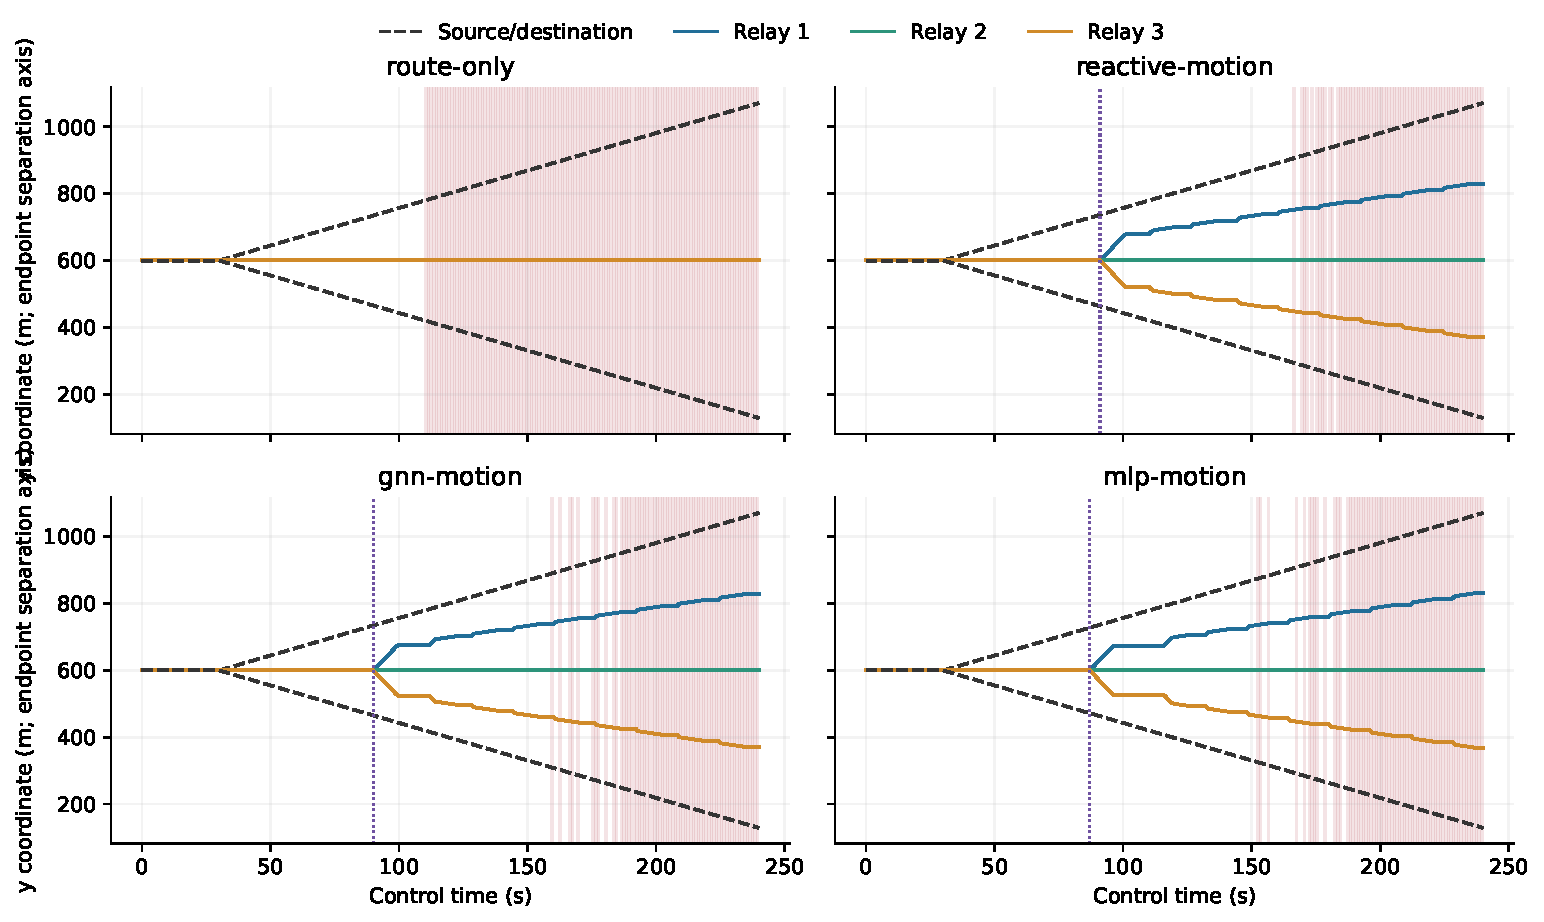
\includegraphics[width=\linewidth]{images/fig_v9_motion_example.pdf}\caption{The n5 gradual episode with the smallest layout seed, shown for all four arms; pale red bands mark probe-graph disconnection and the purple line marks the first commanded motion. The seed was not chosen for a favourable result.}\label{fig:motionexample}\end{figure}

Figure~\ref{fig:motionexample} illustrates the executed actions; the conclusions
are drawn from all scenario blocks. The number of gradual episodes containing
motion is 40/40 for \code{gnn-motion}, 40/40 for \code{mlp-motion}, 40/40 for
\code{reactive-motion} and 0/40 for \code{route-only}.
